\chapter{Simulations}\label{chap:simulations}
As a part of the thesis we have created and simulated a discrete fractional Gaussian field on the Vicsek set $V_m$. The precise field we have constructed was the one given in \Cref{OneToSimulate}. 
These simulations have had a varying rate of success. We have been able to simulate
\begin{equation}
	X_s^{m}(x) = \sum_{j = 1}^{N_m} \left(\lambda_j^{m}\right)^{-s} \phi_j^{m}(x) w_i
\end{equation} for a reasonable set of $s$-values, but we have encountered a limiting factor in the fact that we are not able to simulate $X_s^{m}$ on the Vicsek set for $m \geq 7$. The reason for this limitation lies in \Cref{discreteMatrix}. 

As stated in the remark for any function $f\colon V_m \to \ree$ we can define a matrix $L_m$ such that
\begin{equation}
	L_mF = \begin{pmatrix}
		\Delta_m f(x_1)\\
		\vdots \\
		\Delta_{m}f(x_{N_m})
	\end{pmatrix}, \quad \text{where } F = \begin{pmatrix}
		f(x_1)\\
		\vdots \\
		f(x_{N_m})
	\end{pmatrix}.
\end{equation}
It is precisely from this matrix $L_m$ we compute the eigenvalues and eigenfunctions of $-\Delta_m$. Note that the amount of points in $V_m$ is $5^{m}\cd 4 +1$ so as $m$ grows this number explodes, see \Cref{TableOfValues}), and there is no clever way to construct the matrix $L_m$. Thus the method of constructing the matrix $L_m$ was simply by constructing the Vicsek set $V_m$ and manually checking each point for neighbours.
\begin{table}[!ht]
	\centering
	\begin{tabular}{|c|c|}
		\hline
		$m$  & $\# V_m$ \\ \hline
		$1$  & $21$\\ \hline
		$2$  & $101$\\ \hline
		$3$  & $501$\\ \hline
		$4$  & $2501$\\ \hline
		$5$  & $12501$\\ \hline
		$6$  & $62501$ \\ \hline
		$7$  & $312501$\\ \hline
		$10$ & $39 062 501$\\ \hline
		$20$ & $3.81\cdot10^{14}$\\ \hline                 
	\end{tabular}
	\caption{Points in $V_m$.}
	\label{TableOfValues}
\end{table}

As we see from \Cref{TableOfValues}, the values explode in size as $m$ grows. The process to check each point is therefore slow. Furthermore the matrix $L_m$ that we construct becomes very large, very fast. Since it needs to hold every permutation of points, $L_m$ becomes a $\left(5^{m}\cd 4 + 1\right) \times \left(5^{m}\cd 4 + 1\right)$ matrix. It does however have the property of a sparse matrix, since there is at most five entries in every column, but for $m= 9$ the matrix still fills well over 1 terrabyte in memory.

Having explained the limitations of the simulation, we will quickly delve into the code that generates the simulations. The code will be explained mathematically for clarity, but the full code can be found at: \\ \url{https://gitfront.io/r/Cataclisem/CxGoTRPqvjoM/GaussianFieldsThesis/}.

\section{Construction of the Vicsek set for simulation}
The construction is done by first generating the first "plus" $V_0 = \cbr{ p_1, p_2, p_3, p_4, p_5}$ where $p_1 = (0,0), \ p_2=(\xi, 0), \ p_3 = (0, -\xi), \ p_4 = (-\xi, 0)$ and $p_5 = (0, \xi)$ for some $\xi > 0$. Then going from $V_0$ to $V_1$ we find the endpoints, the tips of the plus, of $V_0$ and then just add $V_0$ to it. Formally written we have:

Let $V^{(0)}_{m}$ be the endpoints after iteration $m$ and $V_m$ be the points of the Vicsek set after iteration $m$, then we define a recursive function so
\begin{equation}
	V_m = \cbr{y + 2\cdot x : x \in V_{m-1}, y \in V^{(0)}_{m-1}}, \quad \text{and} \quad V^{(0)}_m = \cbr{3y : y \in V^{(0)}_{m-1}}.
\end{equation}
Recall from \Cref{fractionalGaussianFieldDiscrete} that a discrete fractional Gaussian field is a Gaussian vector indexed by $V_m$, since the discrete Laplacian depends on the points being in the same places. Thus if we were to compare two different discrete fields we need to make sure the points are in the same order in the list in Python. Luckily we can use the \verb*|set| function in Python. Since the \verb*|set| function hashes each point, it will put the point in a random place in the set, but it will put the point in the same spot every time, given that $\xi$ and $m$ is the same each time. 

The next step is finding all the neighbours of each point. As stated before, there is no good way to find the neighbours thus this step just iterates over every point. We are therefore going to abuse the symmetry and  that we have constructed the Vicsek set outwards. This means that all points in $V_m$, where $x \underset{m}{\sim} y$, are exactly $\abs{x - y} = \xi$ from each other.
Let $V_{m,p}$ denote the neighbours of a point $p$. We thus have
\begin{equation}
	V_{m,p} = \cbr{x + v \in V_m : x \in V_m, v \in V_0}.
\end{equation}
So we actually just add $\xi$ in every direction and see if the point is contained in $V_m$ and finding the neighbours. In Python, we collect each point along with it neighbours in a dictionary. This is because it provides us with a convenient structure to work with, but also because it allows for efficient lookups since dictionaries in Python are hash maps. So while we add each point and its neighbours to the dictionary, we give each point a name, which is $x_i$ where $i$ denotes its place in the set. So each dictionary entry has the following information: 
\begin{equation}
	\cbr{\text{name: }x_i, \text{ Neighbours: } \cbr{(x_\alpha, y_{\alpha}),\ldots }, \text{ coordinate: } (x_i, y_i)}
\end{equation}

To actually construct the discrete Laplacian matrix we do a \verb*|list comprehension| with parameters exactly as in \Cref{discreteMatrix}. 

With the construction of the Vicsek set, the neighbours of each point and the discrete Laplacian, so we move on to generating the eigenfunctions and eigenvalues.

All the constructions mentioned above can be found in \verb*|code/VicsekSet/VicsekSet.py| and \verb*|code/simulations.py|.

\subsection{Eigenvalues and eigenfunctions}
The way we find eigenvalues is through the \verb*|numpy.linalg.eigh| function. The function is for finding eigenvalues and eigenvectors of real symmetric matrices. Some of the best eigenvalue finding algorithms have a runtime of $O(n^2)$, where $n$ is the number of rows in the matrix. As $5^{m}\cd 4 +1$ is a number that grows fast as $m$ increases $(5^{m}\cd 4 +1)^2$ grows even faster making the algorithm slow as $m$ increases.

The code we are describing can be found in \verb*|simulations.py| line 95-101 and line 114-133. Now the function \verb*|numpy.linalg.eigh| gives us a vector of eigenvalues $v_{\text{eig}}$ and a matrix where each column is an eigenvector $M_{\text{eig}}$, having sizes $5^m\cd4 +1 \times 1$ and $5^m\cd4 +1 \times 5^m\cd4 +1$ respectively. The matrix of eigenvectors is actually also our eigenfunctions, since
\begin{equation}
	-\Delta_m (M_{\text{eig}})_{i, -} = (v_{\text{eig}})_i \cd(M_{\text{eig}})_{i, -}, \quad  \text{so} -\Delta_m (M_{\text{eig}})_{i, j} = (v_{\text{eig}})_i \cd(M_{\text{eig}})_{i, j} = \phi_i(x_j).
\end{equation}
Thus we have both our eigenvalues and functions.

Calculating the discrete field in each point is the exact same as in \Cref{OneToSimulate}, where the white noise $W_i$ is generated by \verb*|numpy.random.standard_normal|. To generate the heat maps we plot our points with \verb*|matplotlib| and lay in a colorbar where the colour value corresponds to the values from $X_s^{m}(x)$ for $x \in V_m$.

\newpage
\section{Simulations on the Vicsek set}
The point of the simulations was of course to show the convergence of $X_{s}^{m}$ to $\widetilde{X_s}$ in distribution, but as we have not been able to simulate much over $m \geq 7$ we don't really see any convergence in distribution. What we can observe instead is that the variance in the fields decreases as $s$ increases.

\begin{figure}[!ht]
	\def\scaleParam{0.55}
	\begin{minipage}[l]{0.49\textwidth}
		\centering 
		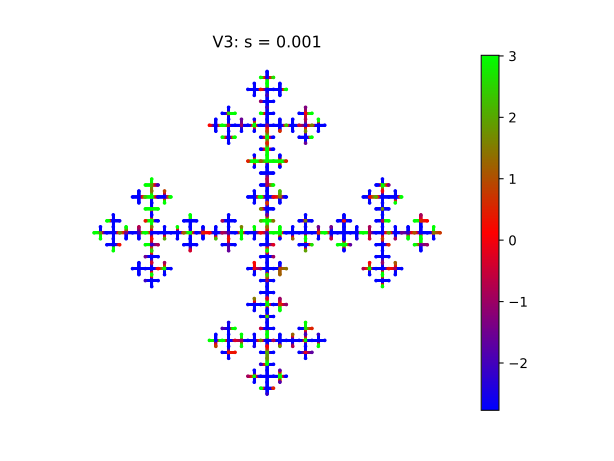
\includegraphics[scale=\scaleParam]{Pictures/vicsekSim/vicsekSim_V3-s0_001.png}
		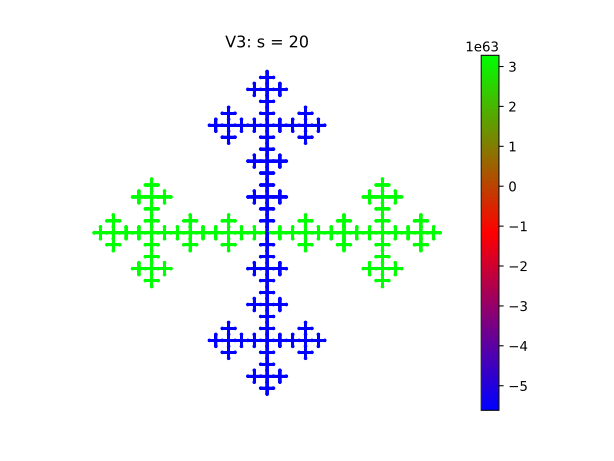
\includegraphics[scale=\scaleParam]{Pictures/vicsekSim/vicsekSim_V3-s20.png}
	\end{minipage}
	\begin{minipage}[r]{0.49\textwidth}
		\centering
		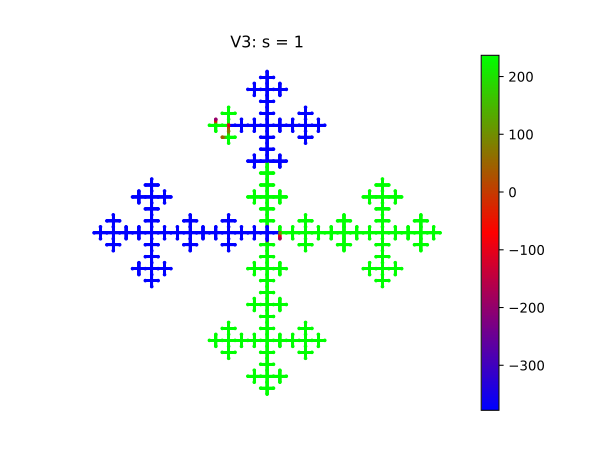
\includegraphics[scale=\scaleParam]{Pictures/vicsekSim/vicsekSim_V3-s1.png}
		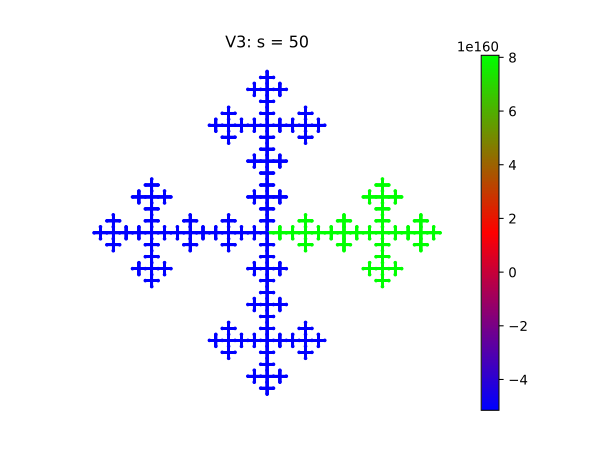
\includegraphics[scale=\scaleParam]{Pictures/vicsekSim/vicsekSim_V3-s50.png}
	\end{minipage}
	\caption{Simulations of the Vicsek set on $V_3$ with different $s$ parameters and 4 different white noise sequences.}
	\label{fig:4differentsSimWithDifferentWhiteNoise}
\end{figure}
\Cref{fig:4differentsSimWithDifferentWhiteNoise} shows 4 different Vicsek sets on $V_3$ each simulated with their own white noise. As can be seen from the values on the colorbar, the fields decrease in variance as $s$ increases. While this is not difficult to see from the definition of $X_s^{m}$, what is interesting is the variance when $s$ is small. If we look at $s = 0.001$, we find that there are many more red spots, meaning there are more transitions between values. 

The figure with $s = 50$ it is very much just green and blue. So they have their extreme values, but looking at the colorbar we discover that the reason that they seem so extreme is because the difference in their values is about $10^{161}$. Hence the field has almost converged to a single value. This again makes sense looking at $X_s^{m}$ where the value $(\lambda_j^{m})^{-s}$ dominates each term as $s$ grows larger.

\medskip
We can further study the influence of the white noise on the simulation. \\
\noi In \Cref{fig:4differentsSimWithSametWhiteNoise} and \Cref{fig:4differentsSimWithSametWhiteNoise2} we have simulated $X_s^{m}$ on $V_3$ for two different sequences of white noise and 4 different values of $s$. If we consider $s = 0.001$ in both \Cref{fig:4differentsSimWithSametWhiteNoise} and \Cref{fig:4differentsSimWithSametWhiteNoise2} we see that the values are quite spread out on the Vicsek fractal. At the value $s = 1$, both figures have have their values be quite far apart, with both of them have their values be $\approx 350 - 400$ apart. But even as they have the extreme values, they are each contained within the same area and do not leave it. As $s = 20$ we see that both figures start to converge towards each other, which makes sense as we argued in the case with \Cref{fig:4differentsSimWithDifferentWhiteNoise}.

A peculiar thing happens as we go from $s = 1$ to $s = 20$. It is that the two blue crosses on the left of the Vicsek set in \Cref{fig:4differentsSimWithSametWhiteNoise} and the small green section on the right of the Vicsek set on \Cref{fig:4differentsSimWithSametWhiteNoise2} both turn into their opposite colour at $s = 20$. This is an effect we cannot quite explain, but we suspect that i might have to do with \emph{floating point errors} as the values in the simulation for $s\geq20$ become very small.

But again the simulations act as we expect, since both $(\lambda_{j}^{m})^{-s}$, which only changes as $s$ changes, and the eigenfunction $\phi_i(x_j)$, with $x_j \in V_m$ will be the same each time. Thus the only change in the fractals are going to be when $w_i$ changes. But since $w_i$ is constant, it follow from the same argument as \Cref{fig:4differentsSimWithDifferentWhiteNoise} that $(\lambda_{j}^{m})^{-s}$ becomes the dominant factor as $s$ changes.
\begin{figure}[!ht]
	\def\scaleParam{0.28}
	\hspace{-3em}
	\begin{minipage}[l]{0.6\textwidth}
		\centering 
		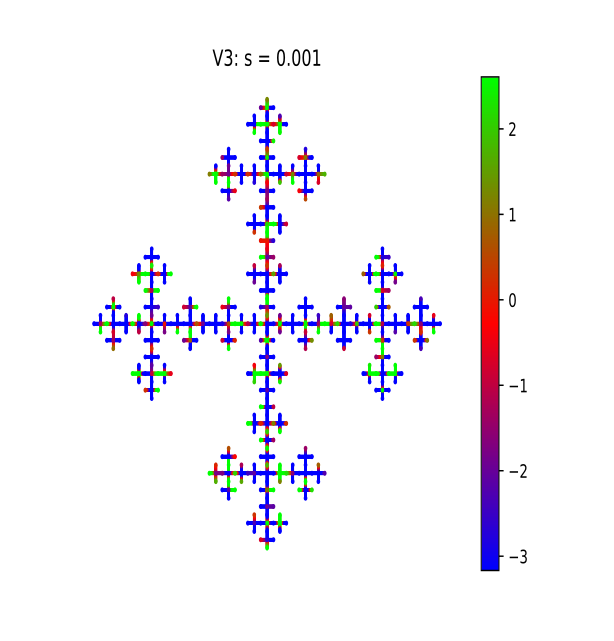
\includegraphics[scale=\scaleParam]{Pictures/vicsekSim/vicsekSim_V3_SameWhiteNoise0-s0_001.png}
		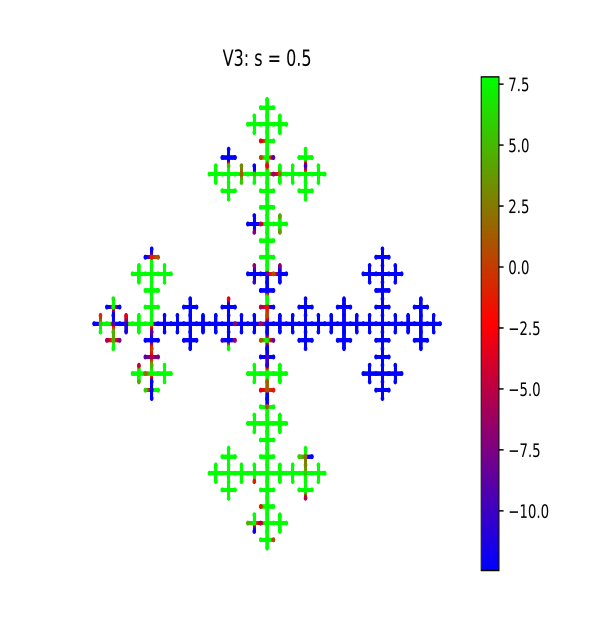
\includegraphics[scale=\scaleParam]{Pictures/vicsekSim/vicsekSim_V3_SameWhiteNoise1-s0_5.png}
	\end{minipage}
	\hspace{-3em}
	\begin{minipage}[r]{0.6\textwidth}
		\centering
		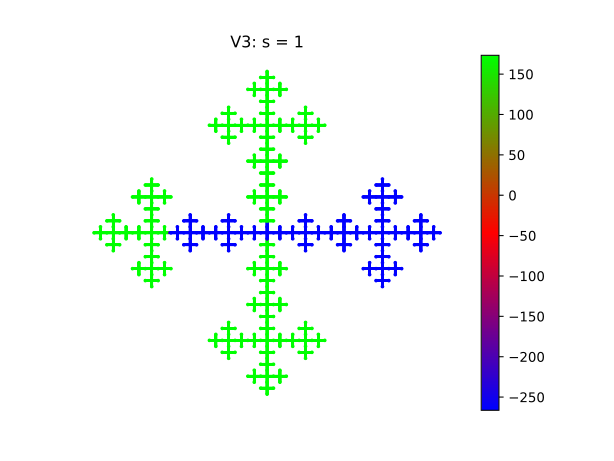
\includegraphics[scale=\scaleParam]{Pictures/vicsekSim/vicsekSim_V3_SameWhiteNoise2-s1.png}
		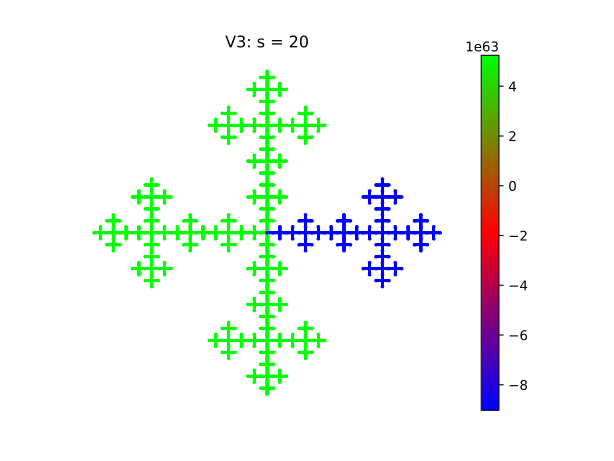
\includegraphics[scale=\scaleParam]{Pictures/vicsekSim/vicsekSim_V3_SameWhiteNoise3-s20.png}
	\end{minipage}
	\caption{Simulations of the Vicsek set on $V_3$ with different $s$ parameters and with the same white noise. A larger version of the image can be found in \Cref{app:SimImages}}
	\label{fig:4differentsSimWithSametWhiteNoise}
\end{figure}

\begin{figure}[!ht]
	\def\scaleParam{0.28}
	\hspace{-3em}
	\begin{minipage}[l]{0.6\textwidth}
		\centering 
		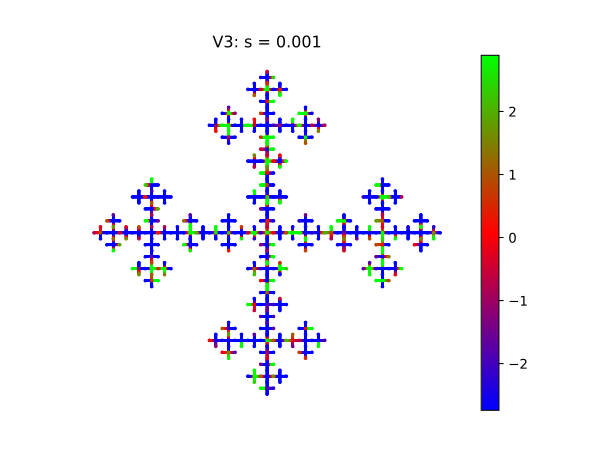
\includegraphics[scale=\scaleParam]{Pictures/vicsekSim/vicsekSim_V3_SameWhiteNoise4-s0_001.png}
		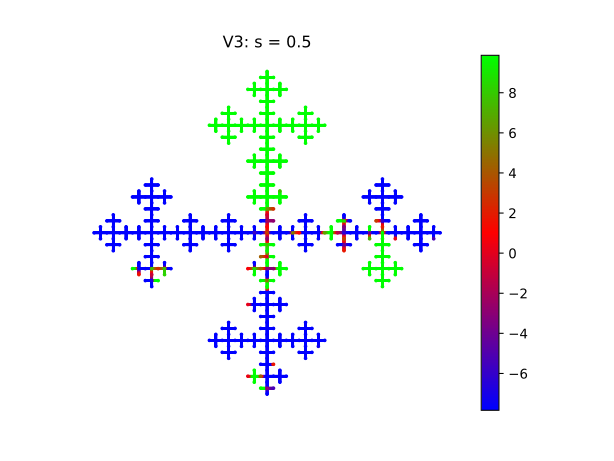
\includegraphics[scale=\scaleParam]{Pictures/vicsekSim/vicsekSim_V3_SameWhiteNoise5-s0_5.png}
	\end{minipage}
	\hspace{-3em}
	\begin{minipage}[r]{0.6\textwidth}
		\centering
		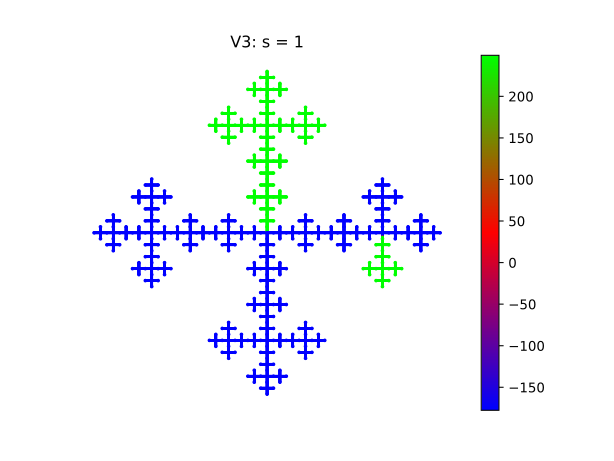
\includegraphics[scale=\scaleParam]{Pictures/vicsekSim/vicsekSim_V3_SameWhiteNoise6-s1.png}
		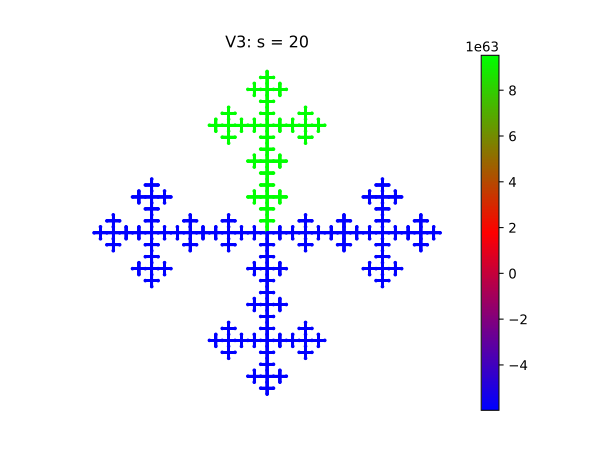
\includegraphics[scale=\scaleParam]{Pictures/vicsekSim/vicsekSim_V3_SameWhiteNoise7-s20.png}
	\end{minipage}
	\caption{Simulations of the Vicsek set on $V_3$ with different $s$ parameters and with the same white noise. A larger version of the image can be found in \Cref{app:SimImages}}
	\label{fig:4differentsSimWithSametWhiteNoise2}
\end{figure}

\newpage
\subsection{Simulations on the Sierpinski gasket}
The described theory in this thesis, is as mentioned before, an extension of the paper \cite{Fabrice} by Fabrice Baudoin and Li Chen. Therefore the theory that made the simulations of the Vicsek set possible also hold for the Sierpinski gasket. Again, we are not able to simulate $m$ very large, but since the amount of points on the Sierpinski gasket is "only" $\frac{3(3^{m} +1 )}{2}$, we are able to simulate $m \leq 11$. The code for  simulations of the Sierpinski gasket are almost identical to the code for the Vicsek set. The main difference being the way the fractal is constructed and the way neighbours are found.  

\vspace{-1em}
\begin{figure}[!ht]
	\def\scaleParam{0.30}
	\begin{minipage}[l]{0.49\textwidth}
		\centering 
		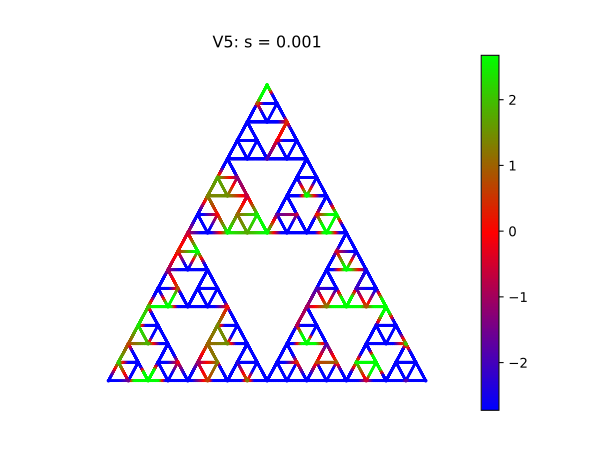
\includegraphics[scale=\scaleParam]{Pictures/sierpinskiSim/sierpinskiSim_V5-s0_001.png}
		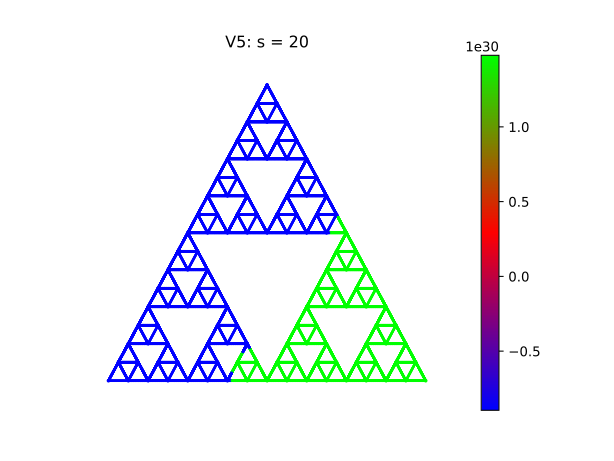
\includegraphics[scale=\scaleParam]{Pictures/sierpinskiSim/sierpinskiSim_V5-s20.png}
	\end{minipage}
	\begin{minipage}[r]{0.49\textwidth}
		\centering
		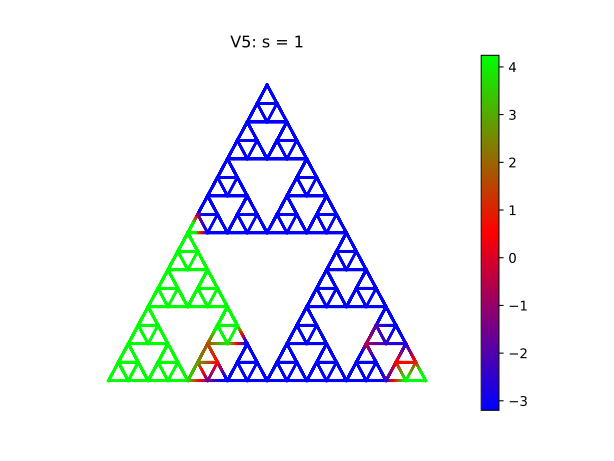
\includegraphics[scale=\scaleParam]{Pictures/sierpinskiSim/sierpinskiSim_V5-s1.png}
		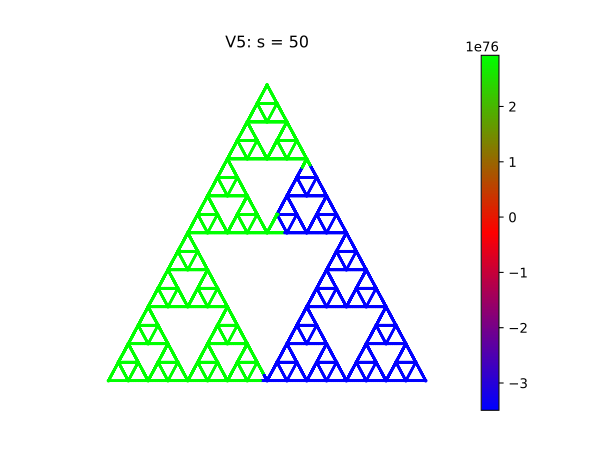
\includegraphics[scale=\scaleParam]{Pictures/sierpinskiSim/sierpinskiSim_V5-s50.png}
	\end{minipage}
	\caption{Simulations of the Sierpinski gasket on $V_5$ with different $s$ parameters and 4 different white noise sequences. A larger version of the image can be found in \Cref{app:SimImages}.}
	\label{fig:Sierpinski4diffWhiteNoise}
\end{figure}

\vspace{-0.7em}
Again we see that in \Cref{fig:Sierpinski4diffWhiteNoise} that the variance converges as $s$ increases, which as explained in the simulations of the Vicsek set, this was to be expected. 

If we again study the influence of white noise in the simulation of the Sierpinski gasket, we see, without surprise, that it behaves almost exactly the same way as the Vicsek set. Precisely that we start with a large variance in the Sierpinski gasket and as $s$ increase the variances tops at $s =1$ and then begins to fall of again as $s$ increases.

\vspace{-0.7em}
\begin{figure}[!ht]
	\def\scaleParam{0.20}
	\hspace{-3em}
	\begin{minipage}[l]{0.6\textwidth}
		\centering 
		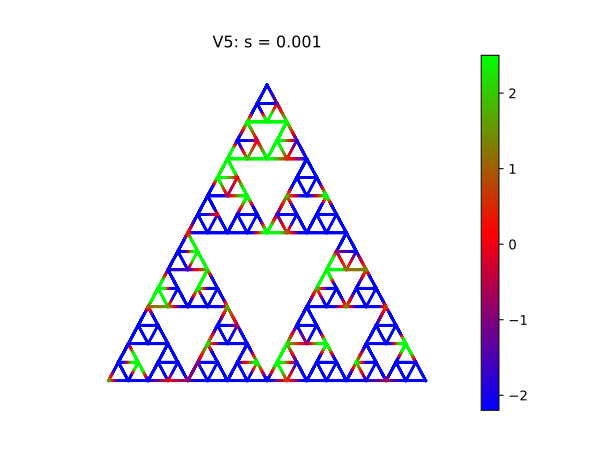
\includegraphics[scale=\scaleParam]{Pictures/sierpinskiSim/sierpinskiSim_V5_SameWhiteNoise0-s0_001.png}
		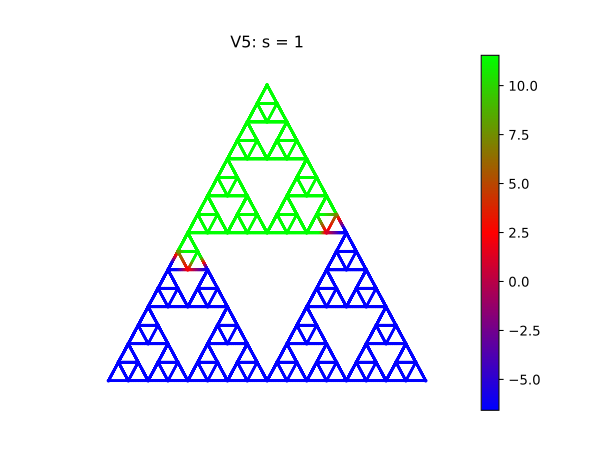
\includegraphics[scale=\scaleParam]{Pictures/sierpinskiSim/sierpinskiSim_V5_SameWhiteNoise2-s1.png}
	\end{minipage}
	\hspace{-3em}
	\begin{minipage}[r]{0.6\textwidth}
		\centering
		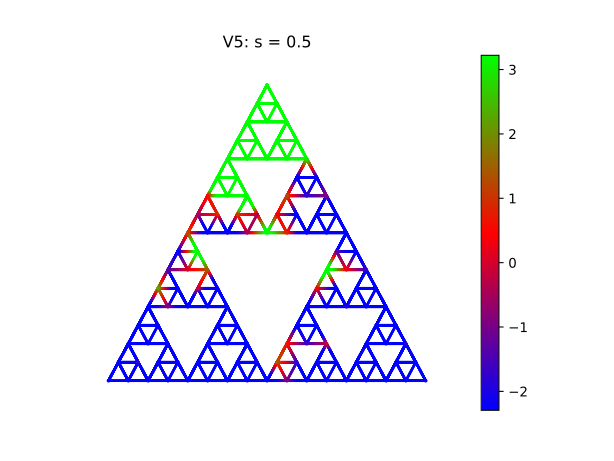
\includegraphics[scale=\scaleParam]{Pictures/sierpinskiSim/sierpinskiSim_V5_SameWhiteNoise1-s0_5.png}
		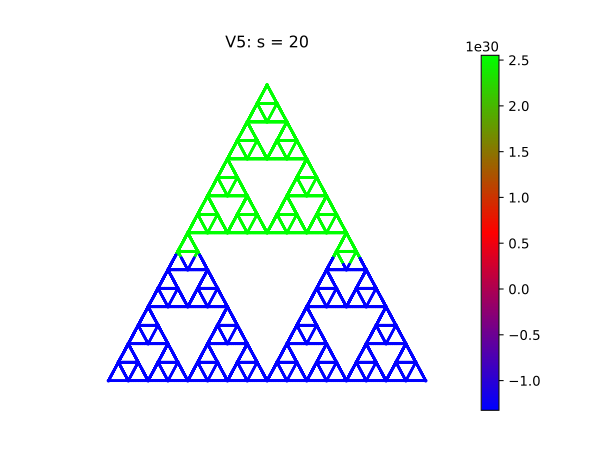
\includegraphics[scale=\scaleParam]{Pictures/sierpinskiSim/sierpinskiSim_V5_SameWhiteNoise3-s20.png}
	\end{minipage}
	\caption{Simulations of the sierpinski gasket on $V_5$ with different $s$ parameters and with the same white noise. A larger version of the image can be found in \Cref{app:SimImages}.}
	\label{fig:sierpinski4differentsSimWithSametWhiteNoise}
\end{figure}

\vspace{-1em}
\begin{figure}[!ht]
	\def\scaleParam{0.20}
	\hspace{-3em}
	\begin{minipage}[l]{0.6\textwidth}
		\centering 
		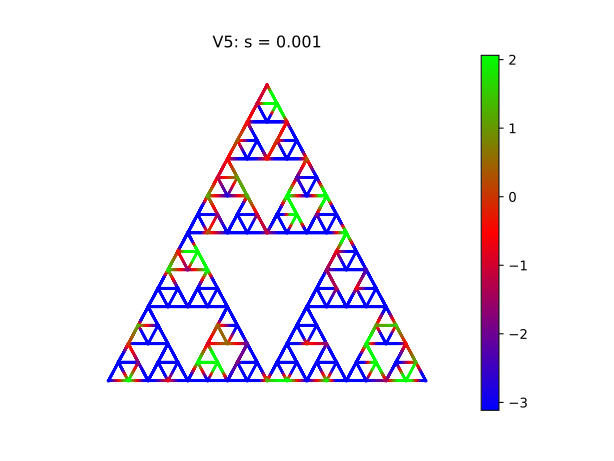
\includegraphics[scale=\scaleParam]{Pictures/sierpinskiSim/sierpinskiSim_V5_SameWhiteNoise4-s0_001.png}
		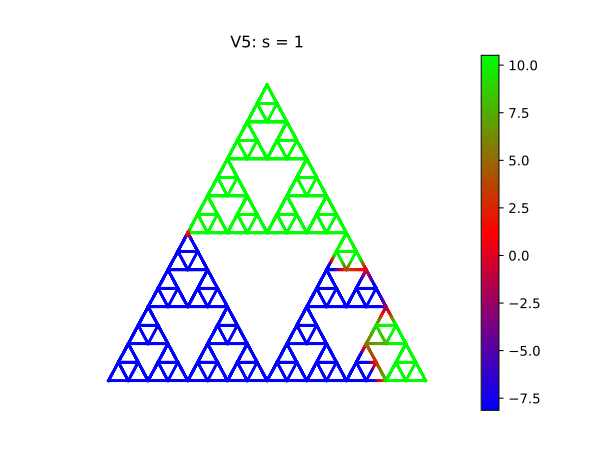
\includegraphics[scale=\scaleParam]{Pictures/sierpinskiSim/sierpinskiSim_V5_SameWhiteNoise6-s1.png}
	\end{minipage}
	\hspace{-3em}
	\begin{minipage}[r]{0.6\textwidth}
		\centering
		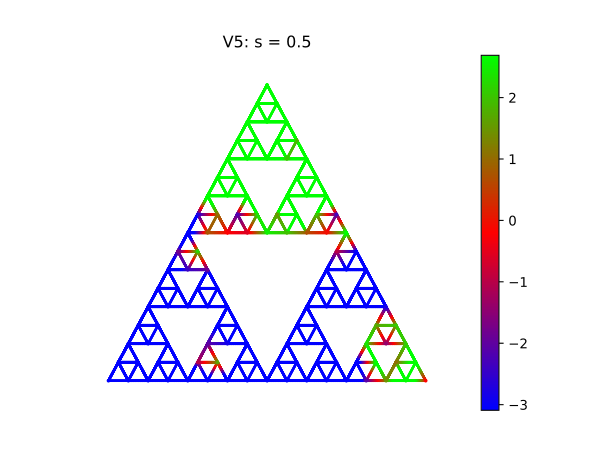
\includegraphics[scale=\scaleParam]{Pictures/sierpinskiSim/sierpinskiSim_V5_SameWhiteNoise5-s0_5.png}
		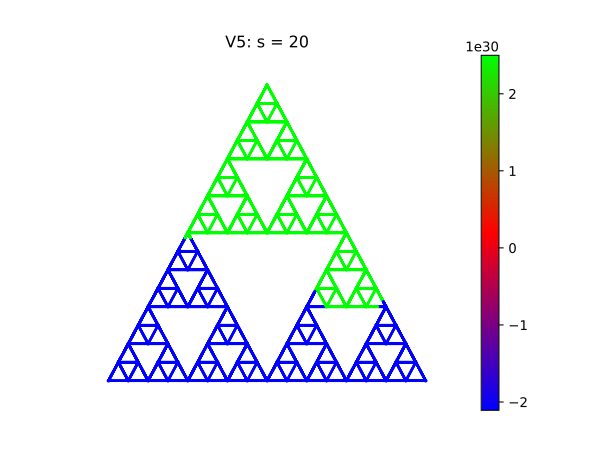
\includegraphics[scale=\scaleParam]{Pictures/sierpinskiSim/sierpinskiSim_V5_SameWhiteNoise7-s20.png}
	\end{minipage}
	\caption{Simulations of the Sierpinski gasket on $V_5$ with different $s$ parameters and with the same white noise. A larger version of the image can be found in \Cref{app:SimImages}}
	\label{fig:sierpniski4differentsSimWithSametWhiteNoise2}
\end{figure}


\section{Conclusion and Future work on the Simulations}

While it was unfortunate that we were not able to show convergence of distribution we were still able to find some points of interest in the simulations. The first being how quickly the simulations converge from quite a varied state. Further, one can see a clear influence of the white noise when observing what values the simulations converge to.

Lastly, the simulations on the Vicsek set and the Sierpinski gasket ended up coinciding, just on different fractals. This is of course what we would expect as the theory behind the simulations is the same. But the construction of the Vicsek set and the Sierpinski gasket could have been different enough to cause some inconsistencies between the two simulations. 

\medskip
Should one wish to continue the work on the simulations, there are two obvious questions to tackle. 

The first being the clustering. Why every simulation ends with the clusters of opposite value, is probably a more mathematical question rather than one that can be answered through computer science. The code should not have any influence on the way that the white noise is chosen, so the clustering might come from a property of the eigenfunctions or eigenvalues. It is of course possible that these clusters are somehow caused by floating point errors as the values in the simulations become very small.

The second question one could tackle is: if a point is encapsulated by points of opposite value why does it suddenly become that value when the simulation progresses. This can be seen in \Cref{fig:4differentsSimWithSametWhiteNoise} and \Cref{fig:4differentsSimWithSametWhiteNoise2} where we have areas that become engulfed by the opposite one. This question relates itself very much to the first question, and one might suspect that finding a solution to the first question will also answer this one. 




